\documentclass[compress]{beamer}
\usepackage[brazil]{babel}
\usepackage[latin1]{inputenc}
\usepackage{amsmath}
\usepackage{graphicx}
\usepackage{color}
\usepackage{colortbl}

%%%%%%%%%%%%%%%%%%%%%%%%%%%%%
% C O N F I G U R A � � E S %
%%%%%%%%%%%%%%%%%%%%%%%%%%%%%

\usetheme{Ilmenau}
\usecolortheme[RGB={176,66,19}]{structure}
\setbeamercovered{transparent}
\setbeamertemplate{footline}[default]
\setbeamertemplate{blocks}[rounded][shadow=true]
\setlength{\tabcolsep}{1mm}
\setbeamertemplate{footline}[frame number]
\setbeamertemplate{navigation symbols}{}

%%%%%%%%%%%
% C A P A %
%%%%%%%%%%%

\title{Proposta de Abordagem Hiperm�dia Adaptativa Baseada em Otimiza��o por Col�nia de Formigas}

\author{Diogo Cezar Teixeira Batista \\
       {\footnotesize \texttt{batista.utfpr@gmail.com}} \\
       Ligia Fl�via Antunes Batista \\
       {\footnotesize \texttt{ligia@utfpr.edu.br}}
}

\institute{\large Universidade Tecnol�gica Federal do Paran� \\
                  Campus Corn�lio Proc�pio \\
                  UTFPR-CP}

\date{Corn�lio Proc�pio - 2007}

\begin{document}

%%%%%%%%%%%%%%%%%%%%%%%%%%%%%%%%
% S L I D E S  I N I C I A I S %
%%%%%%%%%%%%%%%%%%%%%%%%%%%%%%%%

\begin{frame}
    \titlepage
\end{frame}

\begin{frame}[t,allowframebreaks]
    \frametitle{Agenda}
    \tableofcontents
\end{frame}


%%%%%%%%%%%%%%%%%%%%%
% C A P � T U L O S %
%%%%%%%%%%%%%%%%%%%%%

\section[Introdu��o]{Introdu��o}
\begin{frame}
    \frametitle{Introdu��o}
    \begin{itemize}

        \item <1-> Onde est� a p�gina que procuro em um site?

%        \item <1-> Grande n�mero de sistemas hiperm�dia;
%
%        \item <2-> Informa��es distribu�das desorganizadamente na Internet;
%
%        \item <3-> Sistemas de busca;
%
%            \begin{itemize}
%                \item <4-> Trazem conte�do n�o relacionado, ou
%                irrelevante (sem�ntica);
%                \item <5-> N�o oferecem assist�ncia navegacional;
%            \end{itemize}

        \item <2-> \emph{Hiperm�dia Adaptativa}: modifica��o do conte�do
        \emph{web}.

        \item <3-> Proposta: navega��o colaborativa;

            \begin{itemize}
                \item <4-> Ajuda m�tua entre os usu�rios que
                estiverem navegando pelas mesmas p�ginas;

                \item <5-> Solu��o baseada na teoria do comportamento das
                formigas;
            \end{itemize}

    \end{itemize}
\end{frame}

\section[Abordagem de Orienta��o]{Abordagem de Orienta��o}

\begin{frame}
    \frametitle{Intelig�ncia de enxames}

    \begin{itemize}
        \item <1-> Estudos sobre col�nias de insetos (formigas, cupins, abelhas,
        etc);
        \item <2-> Agentes simples interagindo entre si;
        \item <3-> Insetos isoladamente n�o t�m um comportamento
        relevante;
        \item <4-> Em grupo revelam-se uma organiza��o bastante complexa.
    \end{itemize}
\end{frame}

\begin{frame}
    \frametitle{Abordagem de Orienta��o}
    \begin{itemize}

        %\item <1-> capacidade de auto-organiza��o: estigmergia;

        \item <1-> Paradigma de heur�sticas construtivas: \emph{Ant Colony Optimization}
        (ACO) \cite{dorigo:96};

        \item <2-> Formigas reais comunicam-se indiretamente:
        \emph{ferom�nio};

        \item <3-> Fun��o do indiv�duo: procura e o transporte do alimento da fonte at� o
        formigueiro;
        \item <4-> Escolha do caminho: maior quantidade de ferom�nio;
        \item <5-> Em pouco tempo o menor caminho entre origem e
        destino � estabelecido.

    \end{itemize}
\end{frame}

\begin{frame}
    \frametitle{Formigas Reais em Busca de Alimento}

    \begin{figure}[htb]
        \begin{center}
            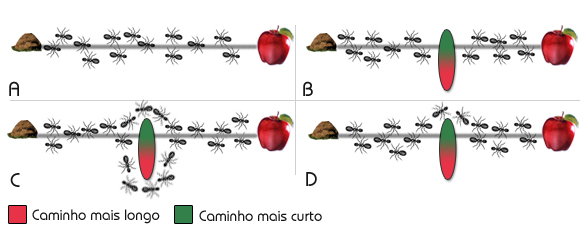
\includegraphics[width=\textwidth]{images/aco/formigas.jpg}
            \caption{Formigas em busca de alimento encontram o menor caminho entre alimento e ninho}
        \end{center}
        \label{fig:formigas}
    \end{figure}

\end{frame}

    \subsection[Hiperm�dia Adaptativa]{Hiperm�dia Adaptativa}

\begin{frame}
    \frametitle{Hiperm�dia Adaptativa}
        \begin{block}{Hiperm�dia Adaptativa}<1->
            A hiperm�dia adaptativa tem como objetivo proporcionar conte�do
            adequado ao perfil ou modelo de cada usu�rio
            \cite{palazzo:02}.
        \end{block}

        Adapta��o dos sistemas hiperm�dia:

        \begin{itemize}
            \item <2-> Adapta��o do conte�do;
            \item <3-> Adapta��o dos links.
        \end{itemize}
\end{frame}

%\begin{frame}
%    \frametitle{M�todos para Navega��o Adaptativa}
%
%        \begin{itemize}
%            \item <1-> condu��o global;
%            \item <2-> condu��o local;
%            \item <3-> suporte � orienta��o global;
%            \item <4-> suporte � orienta��o local;
%        \end{itemize}
%\end{frame}
%
%\begin{frame}
%
%    \frametitle{T�cnicas de Navega��o Adaptativa}
%
%    \begin{itemize}
%        \item <1-> orienta��o direta;
%        \item <2-> classifica��o;
%        \item <3-> oculta��o;
%        \item <4-> anota��o;
%        \item <5-> gera��o de \emph{hyperlinks};
%        \item <6-> mapas adaptativos;
%    \end{itemize}
%\end{frame}

    \subsection[Aplica��o ACO]{Aplica��o ACO}

\begin{frame}
    \frametitle{Aplica��o ACO}

    \begin{itemize}
        \item <1-> Proposta anteriormente proposta \emph{AntWeb} \cite{interlegis};
            \begin{itemize}
                \item <2-> Prot�tipo AntWeb implantado no portal
                Interlegis;
            \end{itemize}
        \item <3-> Limita��o: testes com usu�rios reais;
        \begin{itemize}
            \item <4-> Necess�rio se estabelecer p�gina alvo;
        \end{itemize}
        \item <5-> Abordagem proposta: p�gina alvo determinada pela
        navega��o colaborativa;
    \end{itemize}
\end{frame}

\subsection{Modelo Proposto}

\begin{frame}
    \frametitle{Modelo Proposto}

    Desenvolveu-se um modelo $M<P,G,F>$.

    \begin{block}{Descri��o do modelo}
        \begin{itemize}
            \item P�ginas ($P$);
            \item Grupos ($G$);
            \item Ferom�nio ($F$);
        \end{itemize}
    \end{block}
\end{frame}

\begin{frame}
    \frametitle{Descri��o do Modelo}

        \begin{itemize}
        \item $P$: � uma qu�drupla $P<p, u, e, c>$;
            \begin{itemize}
                \item $p$=identificador; $u$=data e hora do �ltimo
                acesso; $e$=endere�o URL; $c$=n�mero de acessos.
            \end{itemize}

        \item $G$: � uma dupla $G<g, n>$;
            \begin{itemize}
                \item $g$=identificador do grupo; $n$=n�mero de acessos daquele
                grupo.
            \end{itemize}

        \item $F$: � uma qu�drupla $F<o, d, g, qf>$;
            \begin{itemize}
                \item $o$=identificador de
                uma p�gina origem; $d$=identificador da p�gina destino; $g$=identificador de
                grupo; $qf$=quantidade de ferom�nio.
            \end{itemize}

        \end{itemize}
\end{frame}

\begin{frame}
    \frametitle{Acr�scimo de Ferom�nio}

        Para cada acesso, ocorre o acr�scimo de ferom�nio de acordo com a
        equa��o \ref{eq:acrescimo_feromonio}.

        \begin{equation}
            F_{odg} = F_{odg} + \xi
            \label{eq:acrescimo_feromonio}
        \end{equation}

        \emph{onde:}

        \begin{itemize}

            \item $F_{odg}$ � quantidade de ferom�nio na aresta, que liga a origem $o$
            ao destino $d$ para o grupo $g$.

            \item $\xi$ � uma constante definida pelo administrador do sistema, que
            significa a relev�ncia de um acesso.

        \end{itemize}
\end{frame}

\begin{frame}
    \frametitle{Subtra��o de Ferom�nio}

        A f�rmula de subtra��o de ferom�nio foi baseada no conceito de juros
        compostos e pode ser observada na equa��o \ref{eq:reducao}

        \begin{equation}
            \label{eq:reducao}
            F_{odg} = F_{odg} * (1 - \frac{\varphi}{100})^\tau
        \end{equation}

        \emph{onde:}

        \begin{itemize}

            \item $\varphi$ � a taxa de evapora��o de ferom�nio, constante
            definida pelo administrador, dependente do tempo; \\


            \item $\tau$ � o intervalo de tempo, que a p�gina ficou sem acessos,
            determinado pela equa��o~\ref{eq:tau}.

        \end{itemize}

        \begin{equation}
            \tau = t_{atual} - t_{ultimo acesso}
            \label{eq:tau}
        \end{equation}

\end{frame}

    %\subsection{Trabalhos Relacionados}

\begin{frame}
    \frametitle{Trabalhos Relacionados}

       \begin{itemize}

            \item \emph{AntWeb};
            \item modelo de refer�ncia para sistemas hiperm�dia adaptativos
            educacionais; CITAR [5];
            \item abordagem inspirada no comportamento das formigas;
            [12];
            \item metodologia para elabora��o de conte�dos que baseia-se no estilo cognitivo dos
            alunos; [3];
            \item \emph{AdaptWeb}; [7];

        \end{itemize}
\end{frame}

\section{Camada de Adapta��o}

\begin{frame}
    \frametitle{C�lculo da Relev�ncia de uma P�gina}

    \begin{equation}
        \omega(o, d, g) = \frac{F_{odg}}{\sum_{t=1}^{n}F_{otg}}
        \label{eq:relevancia}
    \end{equation}

    \emph{onde:}

    \begin{itemize}
        \item $\omega$ � a relev�ncia daquela p�gina em rela��o �s outras;
        \item $n$ � o n�mero de p�ginas destino a partir daquela
        origem.
    \end{itemize}
\end{frame}

\begin{frame}
    \frametitle{Arquitetura do Modelo Proposto}

    \begin{figure}[htb]
        \begin{center}
            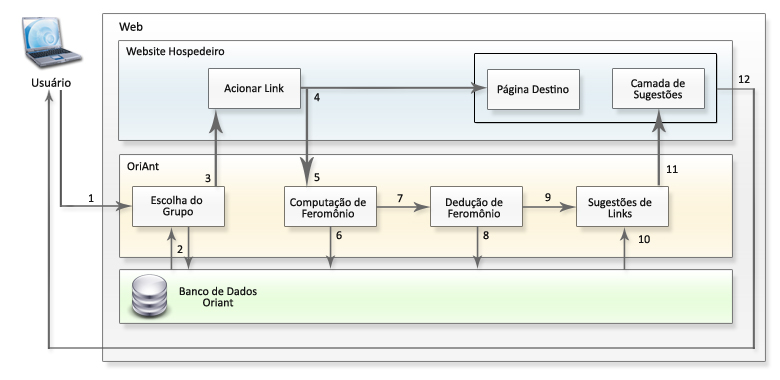
\includegraphics[width=\textwidth]{images/oriant/fig_geral.jpg}
            \label{fig:arquitetura}
            \caption{Arquitetura do modelo proposto}
        \end{center}
    \end{figure}

\end{frame}

\begin{frame}[t,allowframebreaks]
    \frametitle{Op��es para o usu�rio OriAnt}

    \begin{figure}[htb]
        \begin{center}
            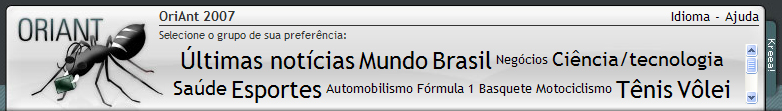
\includegraphics[width=10cm]{images/oriant/grupos.jpg}
            \label{fig:arquitetura}
            \caption{Grupo de interesses}
        \end{center}
    \end{figure}


    \begin{figure}[htb]
        \begin{center}
            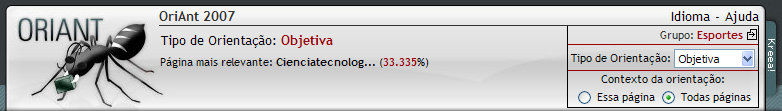
\includegraphics[width=10cm]{images/oriant/objetiva.jpg}
            \label{fig:arquitetura}
            \caption{Disposi��o objetiva}
        \end{center}
    \end{figure}

    \begin{figure}[htb]
        \begin{center}
            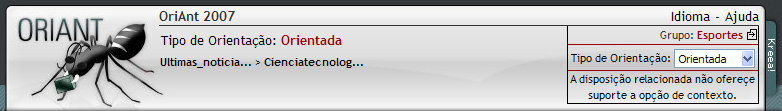
\includegraphics[width=10cm]{images/oriant/orientada.jpg}
            \label{fig:arquitetura}
            \caption{Disposi��o orientada}
        \end{center}
    \end{figure}

    \begin{figure}[htb]
        \begin{center}
            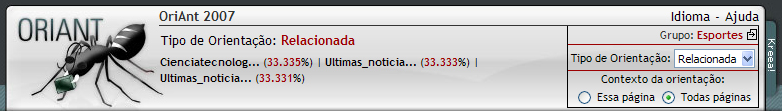
\includegraphics[width=10cm]{images/oriant/relacionada.jpg}
            \label{fig:arquitetura}
            \caption{Disposi��o relacionada}
        \end{center}
    \end{figure}

\end{frame}

\section[Tecnologia]{Tecnologia}

\subsection{Tecnologia}

\begin{frame}
\frametitle{Tecnologia}
    \begin{itemize}
    \item <1-> Linguagem de programa��o: \emph{Hypertext PreProcessor} (PHP);
    \item <2-> Sistemas gerenciadores de banco de dados:
        \begin{itemize}
            \item <3-> PostgreSQL: tabelas do sistema OriAnt;
            \item <4-> MySQL: tabelas do sub-sistema para testes;
        \end{itemize}
    \item <5-> Servidor de aplica��o: Apache 1.33;
    \end{itemize}
\end{frame}

\subsection[Recursos de Desenvolvimento]{Recursos de Desenvolvimento}

\begin{frame}
\frametitle{Recursos de Desenvolvimento}
    Os recursos de desenvolvimento utilizados neste trabalho foram:
    \begin{itemize}
        \item <1-> \emph{Cascading Style Sheets} (CSS);
        \item <2-> Tableless;
        \item <3-> \emph{RDF Site Summary} (RSS);
        \item <4-> \emph{Asynchronous JavaScript and XML} (AJAX);
        \item <5-> Javascript;
    \end{itemize}
\end{frame}

\section[Resultados]{Resultados}

\begin{frame}[t,allowframebreaks]
\frametitle{Resultados}

    Para analisar os resultados, foram realizados tr�s conjuntos de
    testes:

    \begin{enumerate}
        \item links acessados ap�s 1 hora do rein�cio dos registros;
        \item links acessados ap�s 10 horas do rein�cio dos registros;
        \item links acessados ap�s 24 horas do rein�cio dos registros.
    \end{enumerate}

    Para precis�o dos resultados, a equa��o de subtra��o de ferom�nio foi ajustada para
    relevar at� 5 casas decimais.

    \begin{table}
    \centering \caption{Diferen�a de tempo inicial entre as p�ginas}
    \label{tab:diftempo}
    \begin{scriptsize}
    \begin{tabular}{|l|l|l|l|}
    \hline
    pg & �ltimo-acesso & dif & qf0 \\
    \hline
    1 & 12:31 & 0min & 10 \\
    \hline
    2 & 12:31 & 0min & 20 \\
    \hline
    3 & 12:32 & 1min & 10 \\
    \hline
    4 & 12:33 & 2min & 10 \\
    \hline
    5 & 12:35 & 4min & 10 \\
    \hline
    6 & 12:35 & 4min & 20 \\
    \hline
    7 & 12:36 & 5min & 10 \\
    \hline
    8 & 12:36 & 5min & 10 \\
    \hline
    9 & 12:37 & 6min & 10 \\
    \hline
    10 & 12:38 & 7min & 20 \\
    \hline
    11 & 12:39 & 8min & 10 \\
    \hline
    12 & 12:39 & 8min & 10 \\
    \hline
    \end{tabular}
    \end{scriptsize}
    \end{table}

    \newpage

    Os par�metros iniciais do sistema tinham os valores:

    \begin{itemize}
        \item Tr�s grupos de interesse, sendo: 1=�ltimas not�cias; 2=Mundo; 3=Brasil;
        \item Constante que define a relev�ncia de um acesso $\xi$: 10;
        \item Taxa de evapora��o $\varphi$: 35.
    \end{itemize}

\end{frame}

\begin{frame}[t,allowframebreaks]
\frametitle{Links acessados ap�s 1 hora do rein�cio dos registros}

        \begin{table}[H]
        \caption{Links acessados ap�s 1 hora do rein�cio dos registros}
        \label{tab:resultadotr1h}
        \tiny{
            \begin{center}
                \begin{tabular}{|c|c|r|r|r|r|r|r|}
                \hline
                \# & origem-destino-grupo & qf it1 & qf it2 & qf it3 & qf it4 & qf it5 \\
                \hline
                \textcolor[rgb]{0.31,0.51,0.74}{\textbf{1}} & \textcolor[rgb]{0.31,0.51,0.74}{\textbf{1-1-1}} & \textcolor[rgb]{0.31,0.51,0.74}{\textbf{9,92858}} & \textcolor[rgb]{0.31,0.51,0.74}{\textbf{9,85717}} & \textcolor[rgb]{0.31,0.51,0.74}{\textbf{9,78568}} & \textcolor[rgb]{0.31,0.51,0.74}{\textbf{9,71423}} & \textcolor[rgb]{0.31,0.51,0.74}{\textbf{9,64282}} \\
                \hline
                \textcolor[rgb]{0.75,0.31,0.30}{\textbf{2}} & \textcolor[rgb]{0.75,0.31,0.30}{\textbf{1-2-1}} & \textcolor[rgb]{0.75,0.31,0.30}{\textbf{19,85715}} & \textcolor[rgb]{0.75,0.31,0.30}{\textbf{19,71432}} & \textcolor[rgb]{0.75,0.31,0.30}{\textbf{19,57134}} & \textcolor[rgb]{0.75,0.31,0.30}{\textbf{19,42845}} & \textcolor[rgb]{0.75,0.31,0.30}{\textbf{19,28563}} \\
                \hline
                3 & 1-3-1 & 9,92974 & 9,85947 & 9,78911 & 9,71877 & 9,64845 \\
                \hline
                4 & 1-4-1 & 9,9309 & 9,86177 & 9,79253 & 9,72331 & 9,65409 \\
                \hline
                5 & 1-5-2 & 9,93322 & 9,86638 & 9,7994 & 9,7324 & 9,66537 \\
                \hline
                6 & 5-6-2 & 19,86644 & 19,73277 & 19,59881 & 19,46482 & 19,33076 \\
                \hline
                7 & 5-7-2 & 9,93438 & 9,86869 & 9,80284 & 9,73696 & 9,67103 \\
                \hline
                8 & 5-8-2 & 9,93438 & 9,86869 & 9,80284 & 9,73696 & 9,67103 \\
                \hline
                9 & 1-9-3 & 20 & 19,99899 & 19,99677 & 19,99358 & 19,98937 \\
                \hline
                \textcolor[rgb]{0.61,0.73,0.35}{\textbf{10}} & \textcolor[rgb]{0.61,0.73,0.35}{\textbf{9-10-3}} & \textcolor[rgb]{0.61,0.73,0.35}{\textbf{19,8734}} & \textcolor[rgb]{0.61,0.73,0.35}{\textbf{19,7466}} & \textcolor[rgb]{0.61,0.73,0.35}{\textbf{19,61943}} & \textcolor[rgb]{0.61,0.73,0.35}{\textbf{19,49213}} & \textcolor[rgb]{0.61,0.73,0.35}{\textbf{19,36467}} \\
                \hline
                11 & 9-11-3 & 9,93786 & 9,87561 & 9,81316 & 9,75063 & 9,688 \\
                \hline
                12 & 9-12-3 & 9,93786 & 9,87561 & 9,81316 & 9,75063 & 9,688 \\
                \hline
                13 & 9-13-3 & 0 & 10 & 9,9994 & 9,99831 & 9,99671 \\
                \hline
                14 & 9-14-3 & 0 & 0 & 10 & 9,99951 & 9,99852 \\
                \hline
                \textcolor[rgb]{0.49,0.38,0.63}{\textbf{15}} & \textcolor[rgb]{0.49,0.38,0.63}{\textbf{9-15-3}} & \textcolor[rgb]{0.49,0.38,0.63}{\textbf{0}} & \textcolor[rgb]{0.49,0.38,0.63}{\textbf{0}} & \textcolor[rgb]{0.49,0.38,0.63}{\textbf{0}} & \textcolor[rgb]{0.49,0.38,0.63}{\textbf{10}} & \textcolor[rgb]{0.49,0.38,0.63}{\textbf{9,99949}} \\
                \hline
                16 & 9-16-3 & 0 & 0 & 0 & 0 & 10 \\
                \hline
                \end{tabular}
            \end{center}
        }
        \end{table}

        \begin{figure}[htb]
            \begin{center}
                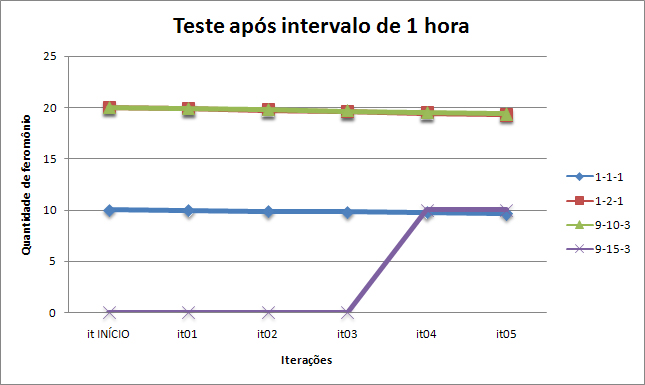
\includegraphics[width=10cm]{images/resultados/qtd_feromonio.jpg}
                \label{fig:qtd_feromonio}
                \caption{Gr�fico dos testes ap�s intervalo de 1 hora}
            \end{center}
        \end{figure}

\end{frame}

\begin{frame}[t,allowframebreaks]
\frametitle{Links acessados ap�s 10 horas do rein�cio dos registros}

        \begin{table}[H]
        \caption{Links acessados ap�s 10 horas do rein�cio dos registros}
        \label{tab:resultadotr10h}
        \tiny{
            \begin{center}
                \begin{tabular}{|c|c|r|r|r|r|r|r|}
                \hline
                \# & origem-destino-grupo & qf it1 & qf it2 & qf it3 & qf it4 & qf it5 \\
                \hline
                \textcolor[rgb]{0.31,0.51,0.74}{\textbf{1}} & \textcolor[rgb]{0.31,0.51,0.74}{\textbf{1-1-1}} & \textcolor[rgb]{0.31,0.51,0.74}{\textbf{9,31582}} & \textcolor[rgb]{0.31,0.51,0.74}{\textbf{8,67811}} & \textcolor[rgb]{0.31,0.51,0.74}{\textbf{8,08376}} & \textcolor[rgb]{0.31,0.51,0.74}{\textbf{7,5296}} & \textcolor[rgb]{0.31,0.51,0.74}{\textbf{7,01306}} \\
                \hline
                \textcolor[rgb]{0.75,0.31,0.30}{\textbf{2}} & \textcolor[rgb]{0.75,0.31,0.30}{\textbf{1-2-1}} &\textcolor[rgb]{0.75,0.31,0.30}{\textbf{18,63165}} & \textcolor[rgb]{0.75,0.31,0.30}{\textbf{17,35624}} & \textcolor[rgb]{0.75,0.31,0.30}{\textbf{16,16754}} & \textcolor[rgb]{0.75,0.31,0.30}{\textbf{15,05922}} & \textcolor[rgb]{0.75,0.31,0.30}{\textbf{14,02614}} \\
                \hline
                3 & 1-3-1 & 9,31691 & 8,68014 & 8,0866 & 7,53313 & 7,01717 \\
                \hline
                4 & 1-4-1 & 9,318 & 8,68217 & 8,08943 & 7,53664 & 7,02126 \\
                \hline
                5 & 1-5-2 & 9,32018 & 8,68624 & 8,09512 & 7,54371 & 7,02949 \\
                \hline
                6 & 5-6-2 & 18,64036 & 17,37247 & 16,19022 & 15,0874 & 14,05896 \\
                \hline
                7 & 5-7-2 & 9,32127 & 8,68827 & 8,09795 & 7,54723 & 7,03359 \\
                \hline
                8 & 5-8-2 & 9,32127 & 8,68827 & 8,09795 & 7,54723 & 7,03359 \\
                \hline
                9 & 1-9-3 & 20 & 19,99922 & 19,9977 & 19,99482 & 19,99089 \\
                \hline
                \textcolor[rgb]{0.61,0.73,0.35}{\textbf{10}} & \textcolor[rgb]{0.61,0.73,0.35}{\textbf{9-10-3}} & \textcolor[rgb]{0.61,0.73,0.35}{\textbf{18,64689}} & \textcolor[rgb]{0.61,0.73,0.35}{\textbf{17,38465}} & \textcolor[rgb]{0.61,0.73,0.35}{\textbf{16,20726}} & \textcolor[rgb]{0.61,0.73,0.35}{\textbf{15,10858}} & \textcolor[rgb]{0.61,0.73,0.35}{\textbf{14,08363}} \\
                \hline
                11 & 9-11-3 & 9,32454 & 8,69436 & 8,10647 & 7,55782 & 7,04593 \\
                \hline
                12 & 9-12-3 & 9,32454 & 8,69436 & 8,10647 & 7,55782 & 7,04593 \\
                \hline
                13 & 9-13-3 & 0 & 10 & 9,99963 & 9,99858 & 9,997 \\
                \hline
                14 & 9-14-3 & 0 & 0 & 10 & 9,99932 & 9,99811 \\
                \hline
                 \textcolor[rgb]{0.49,0.38,0.63}{\textbf{15}} &  \textcolor[rgb]{0.49,0.38,0.63}{\textbf{9-15-3}} &  \textcolor[rgb]{0.49,0.38,0.63}{\textbf{0}} &  \textcolor[rgb]{0.49,0.38,0.63}{\textbf{0}} &  \textcolor[rgb]{0.49,0.38,0.63}{\textbf{0}} &  \textcolor[rgb]{0.49,0.38,0.63}{\textbf{10}} &  \textcolor[rgb]{0.49,0.38,0.63}{\textbf{9,99947}} \\
                \hline
                16 & 9-16-3 & 0 & 0 & 0 & 0 & 10 \\
                \hline
                \end{tabular}
            \end{center}
        }
        \end{table}

        \begin{figure}[htb]
            \begin{center}
                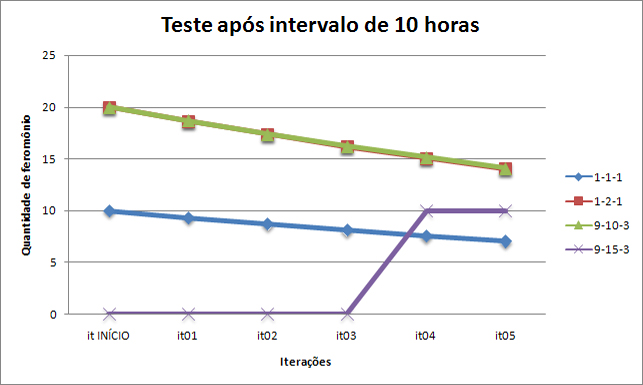
\includegraphics[width=10cm]{images/resultados/graf_teste10h.jpg}
                \label{fig:qtd_feromonio10h}
                \caption{Gr�fico dos testes ap�s intervalo de 10 horas}
            \end{center}
        \end{figure}
\end{frame}

\begin{frame}[t,allowframebreaks]
\frametitle{Links acessados ap�s 24 horas do rein�cio dos registros}

        \begin{table}[H]
        \caption{Links acessados ap�s 24 horas do rein�cio dos registros}
        \label{tab:resultadotr24h}
        \tiny{
            \begin{center}
                \begin{tabular}{|c|c|r|r|r|r|r|r|}
                \hline
                \# & origem-destino-grupo & qf it1 & qf it2 & qf it3 & qf it4 & qf it5 \\
                \hline
                \textcolor[rgb]{0.31,0.51,0.74}{\textbf{1}} & \textcolor[rgb]{0.31,0.51,0.74}{\textbf{1-1-1}} & \textcolor[rgb]{0.31,0.51,0.74}{\textbf{8,39057}} & \textcolor[rgb]{0.31,0.51,0.74}{\textbf{7,03988}} & \textcolor[rgb]{0.31,0.51,0.74}{\textbf{5,90639}} & \textcolor[rgb]{0.31,0.51,0.74}{\textbf{4,95517}} & \textcolor[rgb]{0.31,0.51,0.74}{\textbf{4,15693}} \\
                \hline
                \textcolor[rgb]{0.75,0.31,0.30}{\textbf{2}} & \textcolor[rgb]{0.75,0.31,0.30}{\textbf{1-2-1}} & \textcolor[rgb]{0.75,0.31,0.30}{\textbf{16,78114}} & \textcolor[rgb]{0.75,0.31,0.30}{\textbf{14,07976}} & \textcolor[rgb]{0.75,0.31,0.30}{\textbf{11,81278}} & \textcolor[rgb]{0.75,0.31,0.30}{\textbf{9,91034}} & \textcolor[rgb]{0.75,0.31,0.30}{\textbf{8,31387}} \\
                \hline
                3 & 1-3-1 & 8,39155 & 7,04153 & 5,90846 & 4,95749 & 4,15937 \\
                \hline
                4 & 1-4-1 & 8,39253 & 7,04317 & 5,91053 & 4,9598 & 4,16179 \\
                \hline
                5 & 1-5-2 & 8,3945 & 7,04647 & 5,91468 & 4,96445 & 4,16667 \\
                \hline
                6 & 5-6-2 & 16,78899 & 14,09293 & 11,82936 & 9,92889 & 8,33332 \\
                \hline
                4 & 5-7-2 & 8,39548 & 7,04812 & 5,91676 & 4,96677 & 4,1691 \\
                \hline
                7 & 5-8-2 & 8,39548 & 7,04812 & 5,91676 & 4,96677 & 4,1691 \\
                \hline
                8 & 1-9-3 & 20 & 19,99918 & 19,99758 & 19,99505 & 19,99151 \\
                \hline
                \textcolor[rgb]{0.61,0.73,0.35}{\textbf{10}} & \textcolor[rgb]{0.61,0.73,0.35}{\textbf{9-10-3}} & \textcolor[rgb]{0.61,0.73,0.35}{\textbf{16,79488}} & \textcolor[rgb]{0.61,0.73,0.35}{\textbf{14,10282}} & \textcolor[rgb]{0.61,0.73,0.35}{\textbf{11,84181}} & \textcolor[rgb]{0.61,0.73,0.35}{\textbf{9,94283}} & \textcolor[rgb]{0.61,0.73,0.35}{\textbf{8,34795}} \\
                \hline
                11 & 9-11-3 & 8,39842 & 7,05306 & 5,92298 & 4,97374 & 4,17642 \\
                \hline
                12 & 9-12-3 & 8,39842 & 7,05306 & 5,92298 & 4,97374 & 4,17642 \\
                \hline
                13 & 9-13-3 & 0 & 10 & 9,99961 & 9,99875 & 9,99739 \\
                \hline
                14 & 9-14-3 & 0 & 0 & 10 & 9,99953 & 9,99856 \\
                \hline
                 \textcolor[rgb]{0.49,0.38,0.63}{\textbf{15}} &  \textcolor[rgb]{0.49,0.38,0.63}{\textbf{9-15-3}} &  \textcolor[rgb]{0.49,0.38,0.63}{\textbf{0}} &  \textcolor[rgb]{0.49,0.38,0.63}{\textbf{0}} &  \textcolor[rgb]{0.49,0.38,0.63}{\textbf{0}} &  \textcolor[rgb]{0.49,0.38,0.63}{\textbf{10}} &  \textcolor[rgb]{0.49,0.38,0.63}{\textbf{9,99949}} \\
                \hline
                16 & 9-16-3 & 0 & 0 & 0 & 0 & 10 \\
                \hline
                \end{tabular}
            \end{center}
        }
        \end{table}

        \begin{figure}[htb]
            \begin{center}
                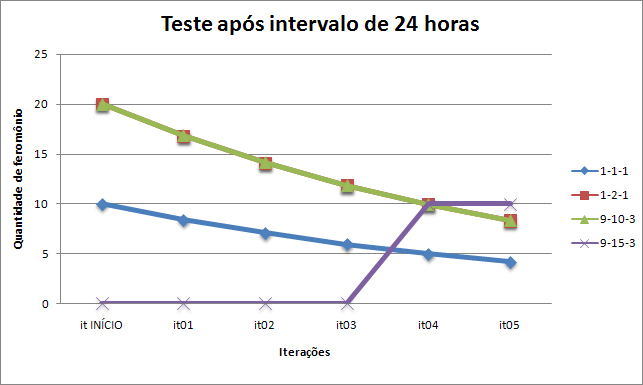
\includegraphics[width=10cm]{images/resultados/graf_teste24h.jpg}
                \label{fig:qtd_feromonio24h}
                \caption{Gr�fico dos testes ap�s intervalo de 24 horas}
            \end{center}
        \end{figure}
\end{frame}

\begin{frame}[t,allowframebreaks]
\frametitle{Diferen�a de ferom�nio nos testes efetuados}

        \begin{table}[H]
        \caption{Diferen�a de ferom�nio nos testes efetuados}
        \label{tab:testesdiferencas}
        \tiny{
            \begin{center}
            \begin{tabular}{|l|l|l|l|l|l|}
            \hline
            \multicolumn{1}{|c|}{Origem} & \multicolumn{1}{c|}{Destino} & \multicolumn{1}{c|}{Grupo} & \multicolumn{1}{c|}{dif 1h} & \multicolumn{1}{c|}{dif 10h} & \multicolumn{1}{c|}{dif 24h} \\
            \hline
            \multicolumn{1}{|c|}{1} & \multicolumn{1}{c|}{1} & \multicolumn{1}{c|}{1} & \multicolumn{1}{c|}{0,32939} & \multicolumn{1}{c|}{2,27586} & \multicolumn{1}{c|}{4,18039} \\
            \hline
            \multicolumn{1}{|c|}{1} & \multicolumn{1}{c|}{2} & \multicolumn{1}{c|}{1} & \multicolumn{1}{c|}{0,65876} & \multicolumn{1}{c|}{4,55171} & \multicolumn{1}{c|}{8,36076} \\
            \hline
            \multicolumn{1}{|c|}{1} & \multicolumn{1}{c|}{3} & \multicolumn{1}{c|}{1} & \multicolumn{1}{c|}{0,32939} & \multicolumn{1}{c|}{2,27586} & \multicolumn{1}{c|}{4,18039} \\
            \hline
            \multicolumn{1}{|c|}{1} & \multicolumn{1}{c|}{4} & \multicolumn{1}{c|}{1} & \multicolumn{1}{c|}{0,32939} & \multicolumn{1}{c|}{2,27586} & \multicolumn{1}{c|}{4,18039} \\
            \hline
            \multicolumn{1}{|c|}{1} & \multicolumn{1}{c|}{5} & \multicolumn{1}{c|}{2} & \multicolumn{1}{c|}{0,32939} & \multicolumn{1}{c|}{2,27586} & \multicolumn{1}{c|}{4,18039} \\
            \hline
            \multicolumn{1}{|c|}{5} & \multicolumn{1}{c|}{6} & \multicolumn{1}{c|}{2} & \multicolumn{1}{c|}{0,65876} & \multicolumn{1}{c|}{4,55171} & \multicolumn{1}{c|}{8,36076} \\
            \hline
            \multicolumn{1}{|c|}{5} & \multicolumn{1}{c|}{7} & \multicolumn{1}{c|}{2} & \multicolumn{1}{c|}{0,32939} & \multicolumn{1}{c|}{2,27586} & \multicolumn{1}{c|}{4,18039} \\
            \hline
            \multicolumn{1}{|c|}{5} & \multicolumn{1}{c|}{8} & \multicolumn{1}{c|}{2} & \multicolumn{1}{c|}{0,32939} & \multicolumn{1}{c|}{2,27586} & \multicolumn{1}{c|}{4,18039} \\
            \hline
            \multicolumn{1}{|c|}{1} & \multicolumn{1}{c|}{9} & \multicolumn{1}{c|}{3} & \multicolumn{1}{c|}{0,02329} & \multicolumn{1}{c|}{0,01679} & \multicolumn{1}{c|}{0,01317} \\
            \hline
            \multicolumn{1}{|c|}{9} & \multicolumn{1}{c|}{10} & \multicolumn{1}{c|}{3} & \multicolumn{1}{c|}{0,65876} & \multicolumn{1}{c|}{4,55171} & \multicolumn{1}{c|}{8,36076} \\
            \hline
            \multicolumn{1}{|c|}{9} & \multicolumn{1}{c|}{11} & \multicolumn{1}{c|}{3} & \multicolumn{1}{c|}{0,32939} & \multicolumn{1}{c|}{2,27586} & \multicolumn{1}{c|}{4,18039} \\
            \hline
            \multicolumn{1}{|c|}{9} & \multicolumn{1}{c|}{12} & \multicolumn{1}{c|}{3} & \multicolumn{1}{c|}{0,32939} & \multicolumn{1}{c|}{2,27586} & \multicolumn{1}{c|}{4,18039} \\
            \hline
            \end{tabular}
            \end{center}
        }
        \end{table}

        \begin{figure}[htb]
            \begin{center}
                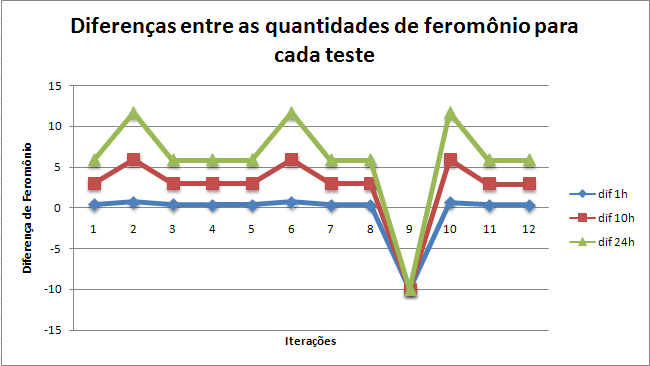
\includegraphics[width=10cm]{images/resultados/graf_diferencas.jpg}
                \label{fig:grafico:dif}
                \caption{Gr�fico indicativo com diferen�a de ferom�nio}
            \end{center}
        \end{figure}

\end{frame}


%%%%%%%%%%%%%%%%%%%%%%%%%%%%%%
% S L I D E S    F I N A I S %
%%%%%%%%%%%%%%%%%%%%%%%%%%%%%%

\section[Refer�ncias]{Refer�ncias}
\begin{frame}[t,allowframebreaks]
    \frametitle{Refer�ncias}
    \nocite{*}
    \bibliographystyle{bst/sbc}
    \tiny \bibliography{bibliografia/bibliografia}
\end{frame}

\begin{frame}
    \begin{center}
    {\Huge D�vidas?} \\
    \vspace{1cm}
    {\LARGE Obrigado pela Aten��o} \\
    {\tiny Apresenta��o desenvolvida em \LaTeX{}} \\
    \vspace{1cm}
    {\normalsize Diogo Cezar Teixeira Batista} \\
    {\footnotesize \texttt{batista.utfpr@gmail.com}} \\
    {\normalsize Ligia Fl�via Antunes Batista} \\
    {\footnotesize \texttt{ligia@utfpr.edu.br}}
    \end{center}
\end{frame}


\end{document}
